\documentclass[12pt]{article}

\usepackage{sbc-template}

\usepackage{graphicx,url}

%\usepackage[latin1]{inputenc}  
\usepackage[brazil]{babel}   
% UTF-8 encoding is recommended by ShareLaTex
\usepackage[utf8]{inputenc}  
\usepackage{float}
\usepackage{wrapfig}

\sloppy

\title{Implementação e análise da estratégia Mutação Seletiva\\para redução de mutantes de primeira ordem}

\author{Alan P. C. Silva\inst{1}}


\address{Departamento de Informática -- Universidade Federal do Paraná (UFPR)\\
  Caixa Postal 19.081 – 81.531-980 – Curitiba – PR – Brazil
  \email{apcs11@inf.ufpr.br}
}

\begin{document} 

\maketitle

\begin{abstract}
  This paper aims to present the Selective Mutation strategy for first ordem 
  mutants reduction and compare it to the methods of production and reduction 
  of high order mutants First to Last, Differente Operators, Random Mix and 
  Each-choice.
\end{abstract}
     
\begin{resumo} 
  Este artigo busca apresentar a estratégia Mutação Seletiva de redução de 
  mutantes de primeira ordem e compará-la aos métodos de produção e redução de 
  mutantes de ordem maior First to Last, Differente Operators, Random Mix e
  Each-choice.
\end{resumo}


\section{Introdução}
\label{section:introduction}
Este estudo apresentará a implementação da estratégia de redução de mutantes
de primeira ordem chamada de Mutação Seletiva, assim como os resultados obtidos
ao ser aplicada em 6 diferentes problemas cujos mutantes de primeira ordem
já foram selecionados e a matriz de resultados dos casos de teste foram 
previamente calculadas.
\section{Metodologia utilizada}
\label{section:UsedMethodology}

Foram executados 6 sistemas implementados em Java já utilizados em outro 
trabalho de \cite{polo2009decreasing}.
Os detalhes dos sistemas  relacionados aos números de linhas de código e
o número de casos de testes foram obtidos usando o plugin Source Code 
Metrics para Netbeans \cite{sourceCodeMetrics2016} e são apresentados
junto ao número de FOMs para cada um na tabela 
(\ref{table:QuantitativeSystemDescription})\footnote{Os casos de teste
e os sistemas utilizados neste trabalho estão acessíveis em 
http://bit.do/SUTs4MutationTesting.}.

\begin{table}[h]
  \label{table:QuantitativeSystemDescription}
  \centering
  \caption{Descrição quantitativa sobre os sistemas}
  \begin{tabular}{|c|c|c|c|} \hline
    Aplicação               & Linhas de código  & Número de casos de teste     & Número de FOMs \\ \hline
    Bisect                  & 35                & 25                           & 198            \\ \hline
    Bub                     & 50                & 256                          & 172            \\ \hline
    Find                    & 62                & 135                          & 299            \\ \hline
    Fourballs               & 42                & 96                           & 292            \\ \hline
    Mid                     & 57                & 125                          & 317            \\ \hline
    Triangulo(TryTip)       & 88                & 216                          & 605            \\ \hline
  \end{tabular}
\end{table}

Os testes usados em todos os sistemas foram implementados no seguinte 
trabalho \cite{polo2009decreasing}.

\subsection{Produção dos FOMs e casos de teste}
A geração foi feita usando a ferramenta MuJava \cite{ma2005mujava}, 
a partir dos mutantes gerados foram criados casos de teste usando JUnit, 
uma biblioteca Java para testes. Os casos de teste gerados foram 
executados sobre os mutantes, resultando em uma matriz cuja combinação 
de linha (mutante) e coluna (caso de teste) contém 0 se o mutante 
não foi morto em 1 caso tenha sido morto.

Para a análise, os FOMs (mutantes de primeira ordem) vivos foram considerados como equivalente para
que o \textit{score}\footnote{O \textit{score} é calculado pela relação: 
(mutantes mortos - (total - equivalentes))/(total - equivalentes)} máximo 
seja inicialmente 1.0, facilitando a comparação entre as estratégias.

\subsection{Produção dos SOMs}
As estratégias utilizadas para produção de SOMs (mutantes de segunda ordem) foram implementados por
Polo\cite{polo2009decreasing} and Mateo\cite{reales2013validating}. Das
estratégias avaliadas foram escolhidas: \textit{FirstToLast}, 
\textit{RandomMix} and \textit{Different-Operators}, definias 
respectivamente por \textit{First2Last}, \textit{Random} e
\textit{DiffOp}. Além dessas 3 estratégias citadas , foi escolhida mais
uma de \cite{reales2013validating}: \textit{Each-Choice}.

Essas abordagens demostram uma redução no número de SOMs gerados
mantendo a eficácia dos testes e foram escolhidas pela facilidade
de produção, implementação e bons resultados obtidos.

\subsection{Mutação seletiva}
O objetivo da mutação seletiva é remover os FOMs gerados pelos \textit{x} 
operadores que mais geraram FOMs, onde \textit{x} é um número inteiro. Uma
abordagem que parece promissora pois como os mutantes são dos operadores 
que mais geraram mutantes, uma quantidade significativa de mutantes
será removida, que por sua vez podem ser mutantes que sejam mortos por muitos
casos de uso, e caso isso se mostre verdade, serão removidos uma parcela
considerável de mutantes, reduzindo o custo computacional de processamento
e mantendo o \textit{score} próximo ao original.

\subsubsection{Implementação}
Para implementar a estratégia de mutação seletiva foi criado um código
em Ruby\footnote{Linguagem de programação dinâmica, mais detalhes 
em: https://www.ruby-lang.org/pt/} que recebe como argumentos:
\begin{enumerate}
\item Diretório raíz dos problemas, por exemplo: 'sources/' (Obrigatório).
\item Conjunto com quantos \textit{x} operadores cujos FOMs serão removidos da 
matriz original, por exemplo: '[2,5,7,6]' (Opcional).
\end{enumerate}

Ao executar o código é criado um arquivo chamado MS\_\textit{X}.csv para cada 
\textit{x} passado no segundo argumento, caso especificado. Caso não seja 
passado o segundo argumento, o programa irá retirar os FOMs gerados 
pelos 2, 5 e 10 operadores que mais geraram FOMs e inserílos em arquivos
 MS\_\textit{X}\_removed.csv para que seja possível também analisar o 
complemento da estratégia seletiva.

Após a aplicação da estratégia, foi executado um programa\footnote{esta 
ferramenta foi desenvolvida utilizando um algoritmo genético de busca
[Féderle, Guizzo, Colanzi, Vergilio e Spinosa, 2013]} que tenta encontrar
o conjunto mínimo de caso de testes que mata a maioria dos mutantes, porém 
como este problema é complexo computacionalmete, este programa retorna um 
conjunto próximo do mínimo, porém não determinístico, e por esse motivo é
executado 10 vezes. Os conjuntos resultantes de cada execução são escritos
em arquivos com prefixo 'testcases\_' para cada um dos resultados de cada
estratégia.

Por fim é executado um outro código em escrito Ruby que recebe como 
argumentos:
\begin{enumerate}
\item Diretório raíz dos problemas, por exemplo: 'sources/' (Obrigatório).
\item '-\--summary' Flag para agrupar por média simples aritmética os scores
por estratégia, e não por conjuntos de caso de teste (Opcional).
\end{enumerate}
Que busca na raíz recebida como parâmetro por arquivos com o prefixo 
'\textit{testcases\_}'. Para cada um dos arquivos, lê os conjuntos de 
casos de teste únicos e para cada um calcula os scores na matriz de FOMs
mortos originais obtendo como saída uma média do score para cada um 
dos arquivos.

Os resultados são impressos na saída padrão em JSON\footnote{JSON é uma
formatação leve de troca de dados, mais detalhes em http://www.json.org/}
de cada uma das estratégias comparando-os aos FOMs mortos originais, 
seus resultados serão apresentados a seguir.
\section{Análise dos resultados}
Nas seções seguintes iremos comparar resultados obtidos ao executar as estratégias HOM e Mutação Seletiva a cada problemas estudado e em seguida o \textit{score} de cada problema por estratégia.

\subsection{Análise por problemas}
Primeiro iremos mostrar o desempenho de cada uma das estratégias em cada um dos seis problemas estudados.

\subsubsection{Bisect}
\begin{figure}[H]
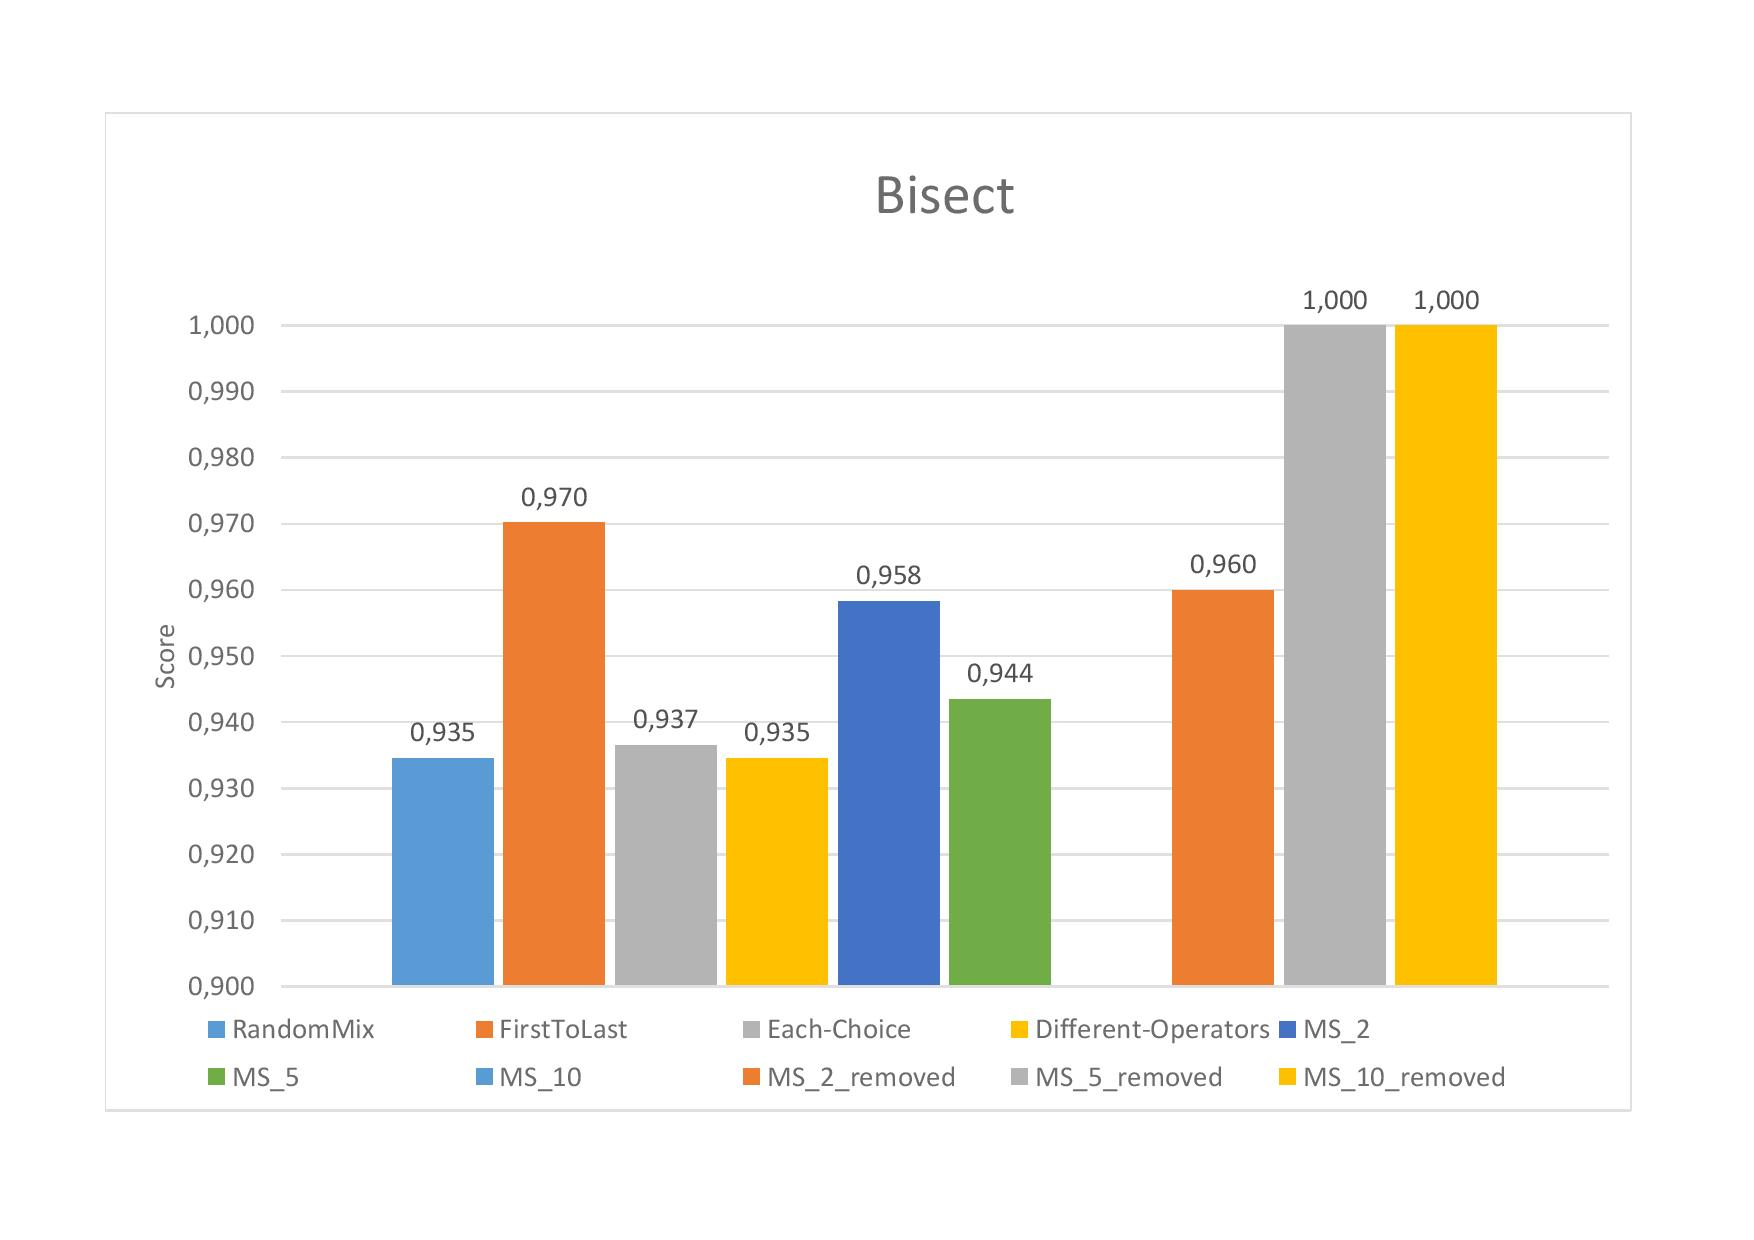
\includegraphics[width=1\textwidth]{graficos/problems/bisect.jpg}
\caption{\textit{Scores} das estratégias no problema Bisect}
\label{fig:bisect}
\end{figure}
No \textit{Bisect} podemos notar que com excessão da MS\_10, as estratégias MS\_2, MS\_5 e MS\_2\_removed se saíram melhores do que 3 dos 4 SOMs. O MS\_2 e seu complemento ganharam com vantagem expressiva aos 3 SOMs.
A estratégia MS\_10 não obteve resultado, isso aconteceu porque a matriz de FOMs fonte possuía mutantes de 10 ou menos operadores, restando nenhum mutante para ser avaliado.

\subsubsection{Bub}
\begin{figure}[H]
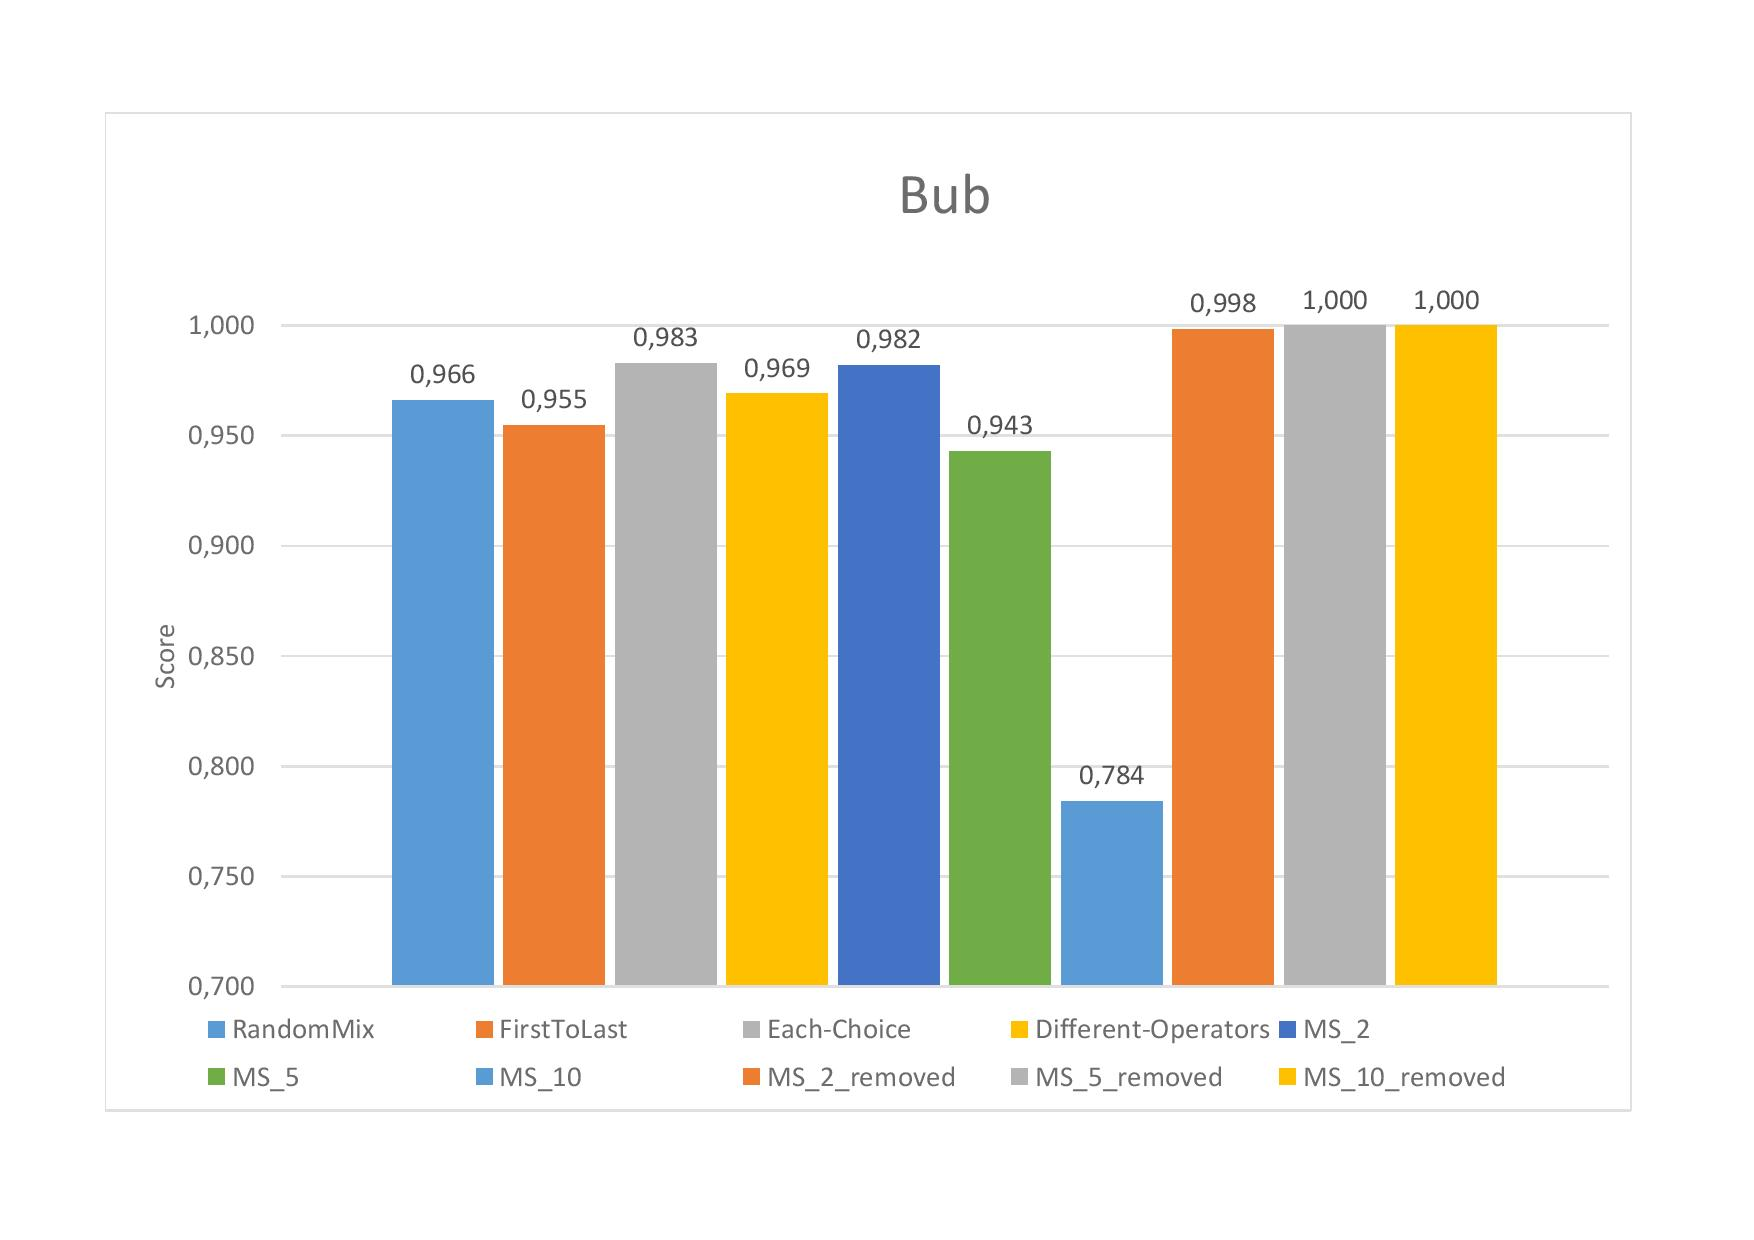
\includegraphics[width=1\textwidth]{graficos/problems/bub.jpg}
\caption{\textit{Scores} das estratégias no problema Bub}
\label{fig:bub}
\end{figure}
No \textit{Bub} podemos notar que novamente o MS\_10 mostrou um desempenho muito abaixo da dos demais e que o MS\_2 praticamente empatou com o SOM que obteve o melhor \textit{score}. Algo a se notar nesse problema, é que os complementos ficaram quase em 1.0, e o MS\_2\_removed, por possui um número menor de mutantes que os demais complementos, começa parecer uma estratégia interessante de se trabalhar.

\subsubsection{Find}
\begin{figure}[H]
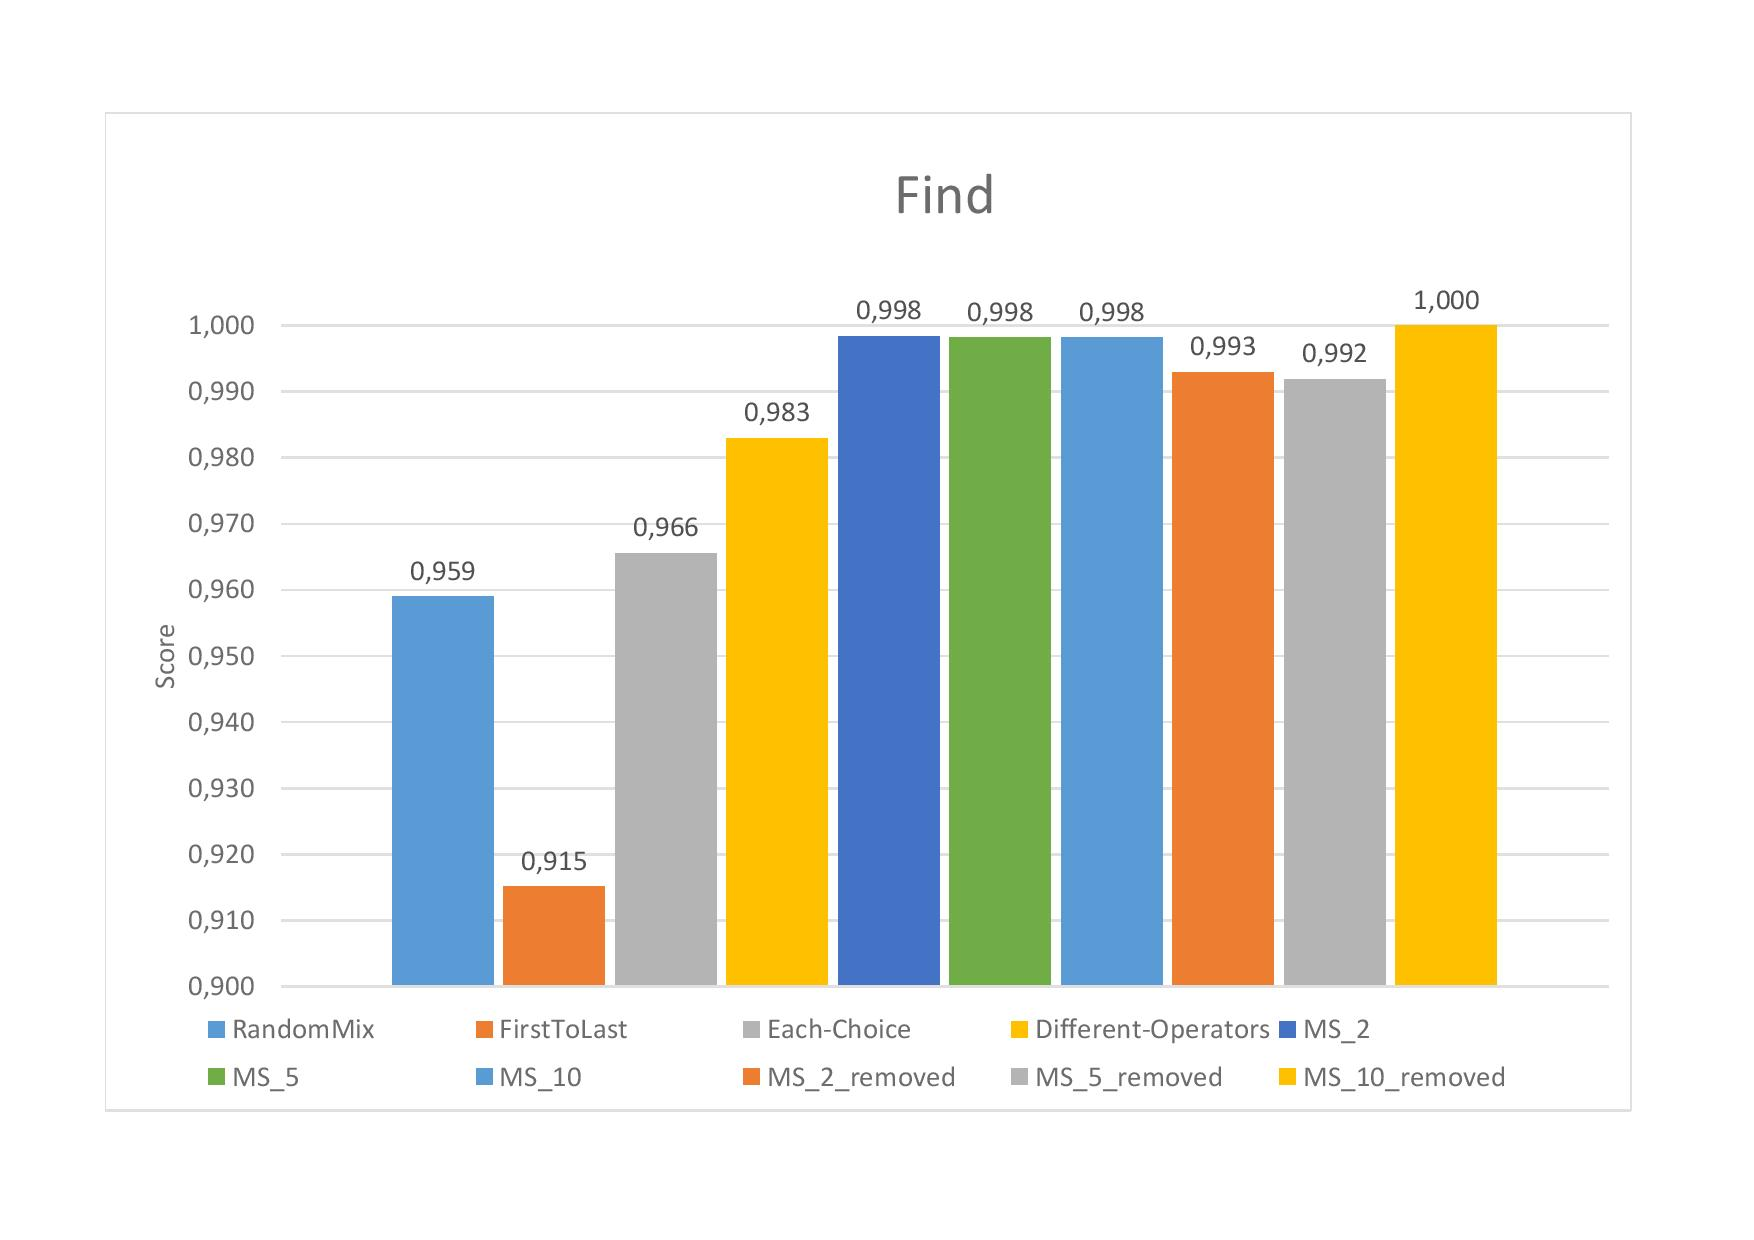
\includegraphics[width=1\textwidth]{graficos/problems/find.jpg}
\caption{\textit{Scores} das estratégias no problema Find}
\label{fig:find}
\end{figure}
Neste problema, todas as estratégias de mutação seletiva se mostraram mais eficazes que os SOMs. Vale lembrar que a estratégia MS\_10 tem um número muito reduzido de FOMs e que a  MS\_2 possui ainda menos, no entanto seus \textit{scores} ainda ficaram próximos ao \textit{score} ideal.

\subsubsection{Fourballs}
\begin{figure}[H]
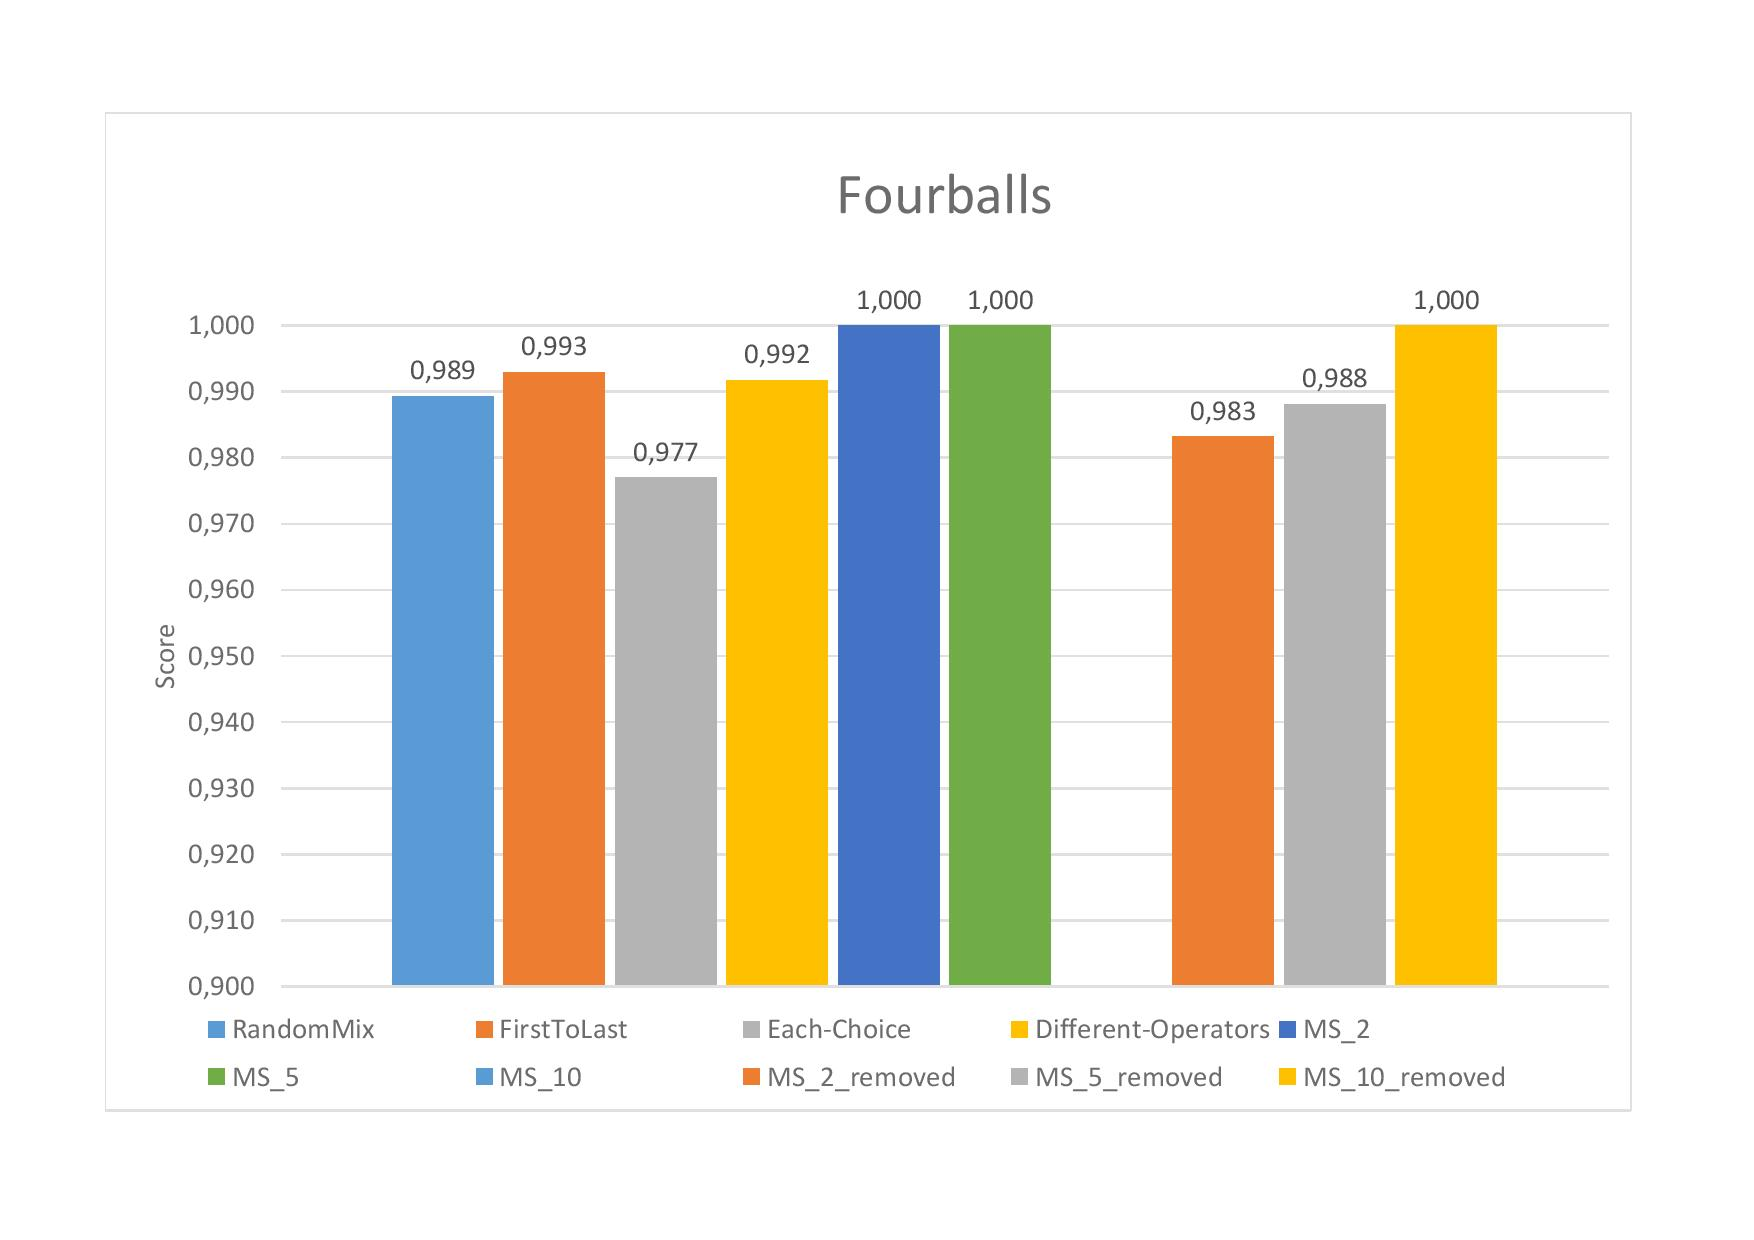
\includegraphics[width=1\textwidth]{graficos/problems/fourballs.jpg}
\caption{\textit{Scores} das estratégias no problema Fourballs}
\label{fig:fourballs}
\end{figure}
No \textit{Fourballs} tanto o MS\_2 quanto MS\_5 obtiveram \textit{score} máximo e seus complementos ficaram próximos dos SOMs estudados, porém como nesse caso temos poucos operadores, a estratégia de mutação seletiva que terá o menor conjunto de mutantes é a MS\_2. 
Novamente a estratégia MS\_10 não obteve resultado porque a matriz de FOMs fonte possuía mutantes de 10 ou menos operadores, restando nenhum mutante para ser avaliado.

\subsubsection{Mid}
\begin{figure}[H]
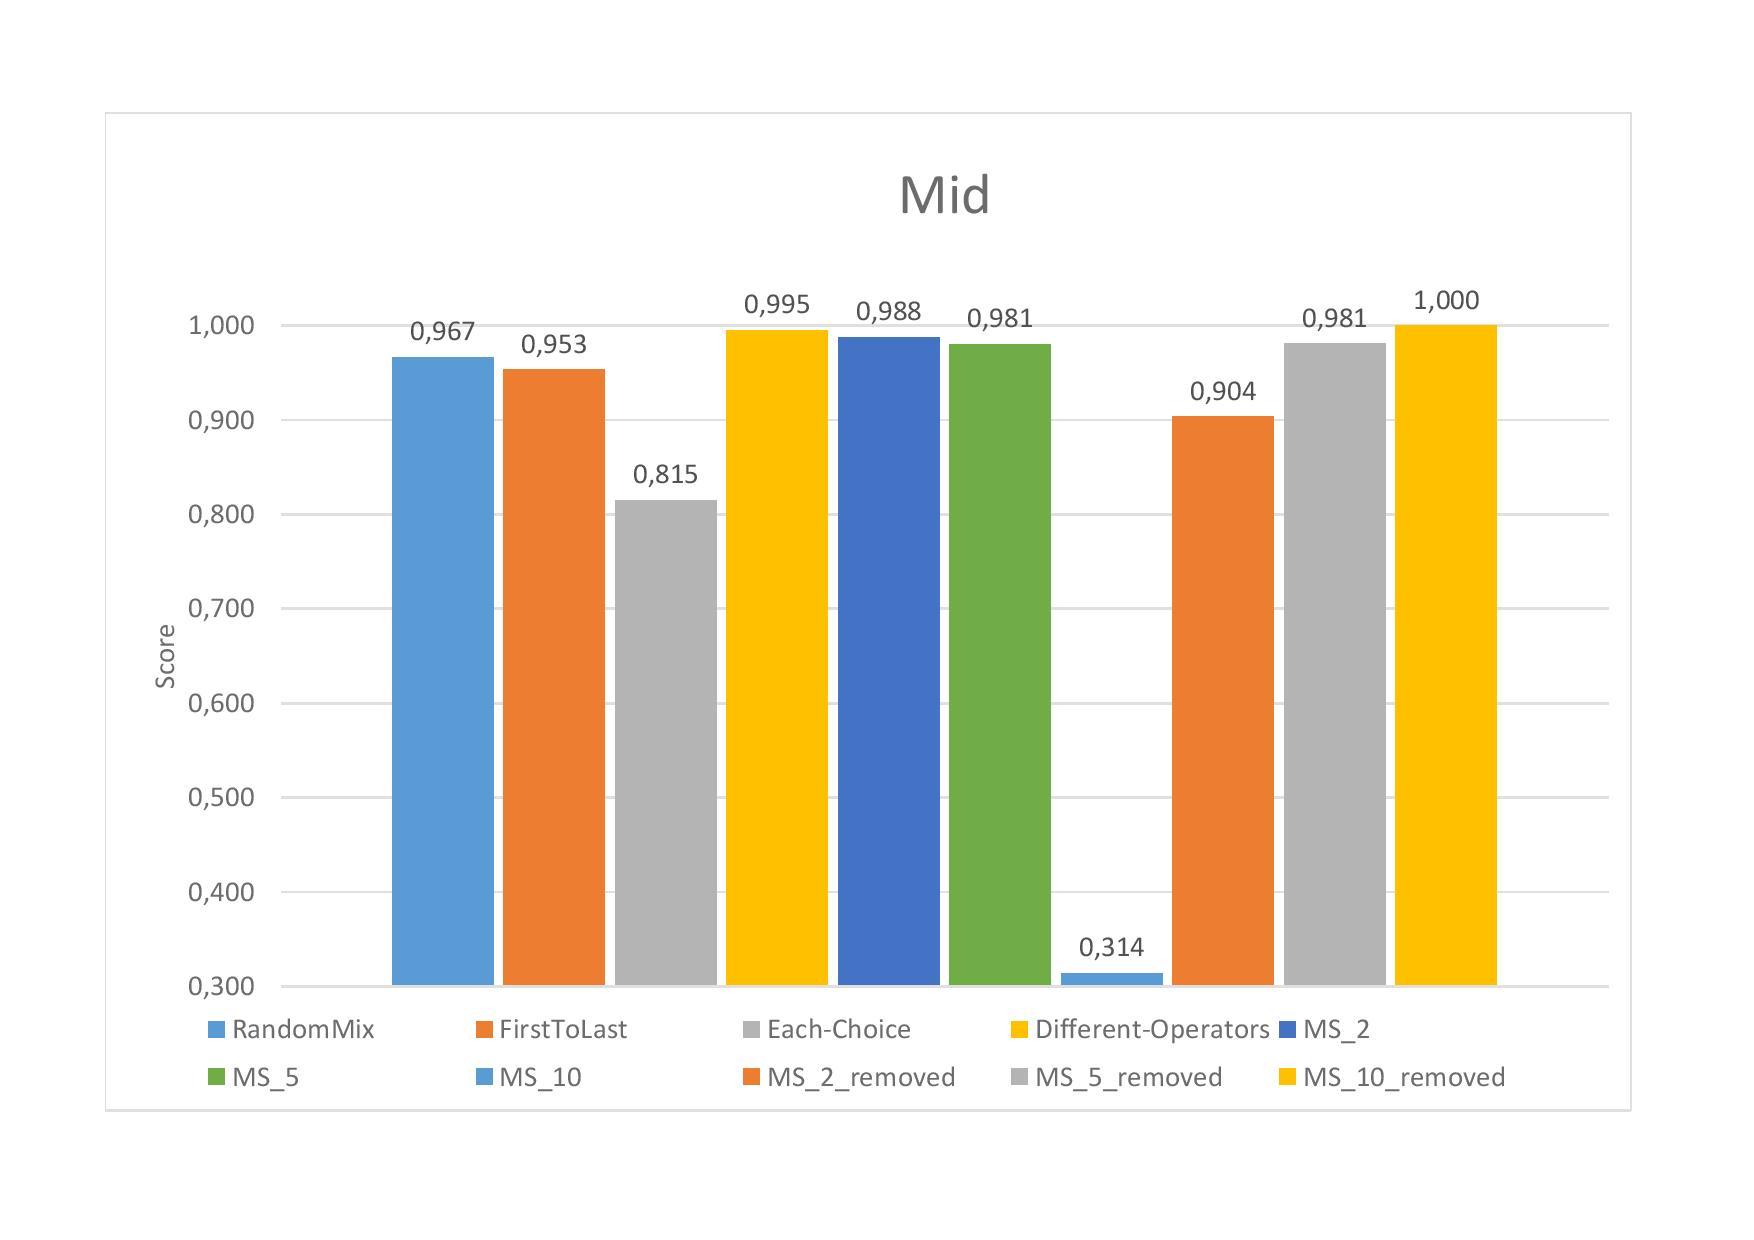
\includegraphics[width=1\textwidth]{graficos/problems/mid.jpg}
\caption{\textit{Scores} das estratégias no problema Mid}
\label{fig:mid}
\end{figure}
A execução para este problema mostra novamente que a estratégia MS\_10 possui um score muito abaixo do ideal, e que as estratégias MS\_2 e MS\_5 novamente se mostraram muito eficientes, perdendo por apenas aproximadamente 0,007 para o SOM \textit{Different-Operators}.
\subsubsection{Triangulo}
\begin{figure}[H]
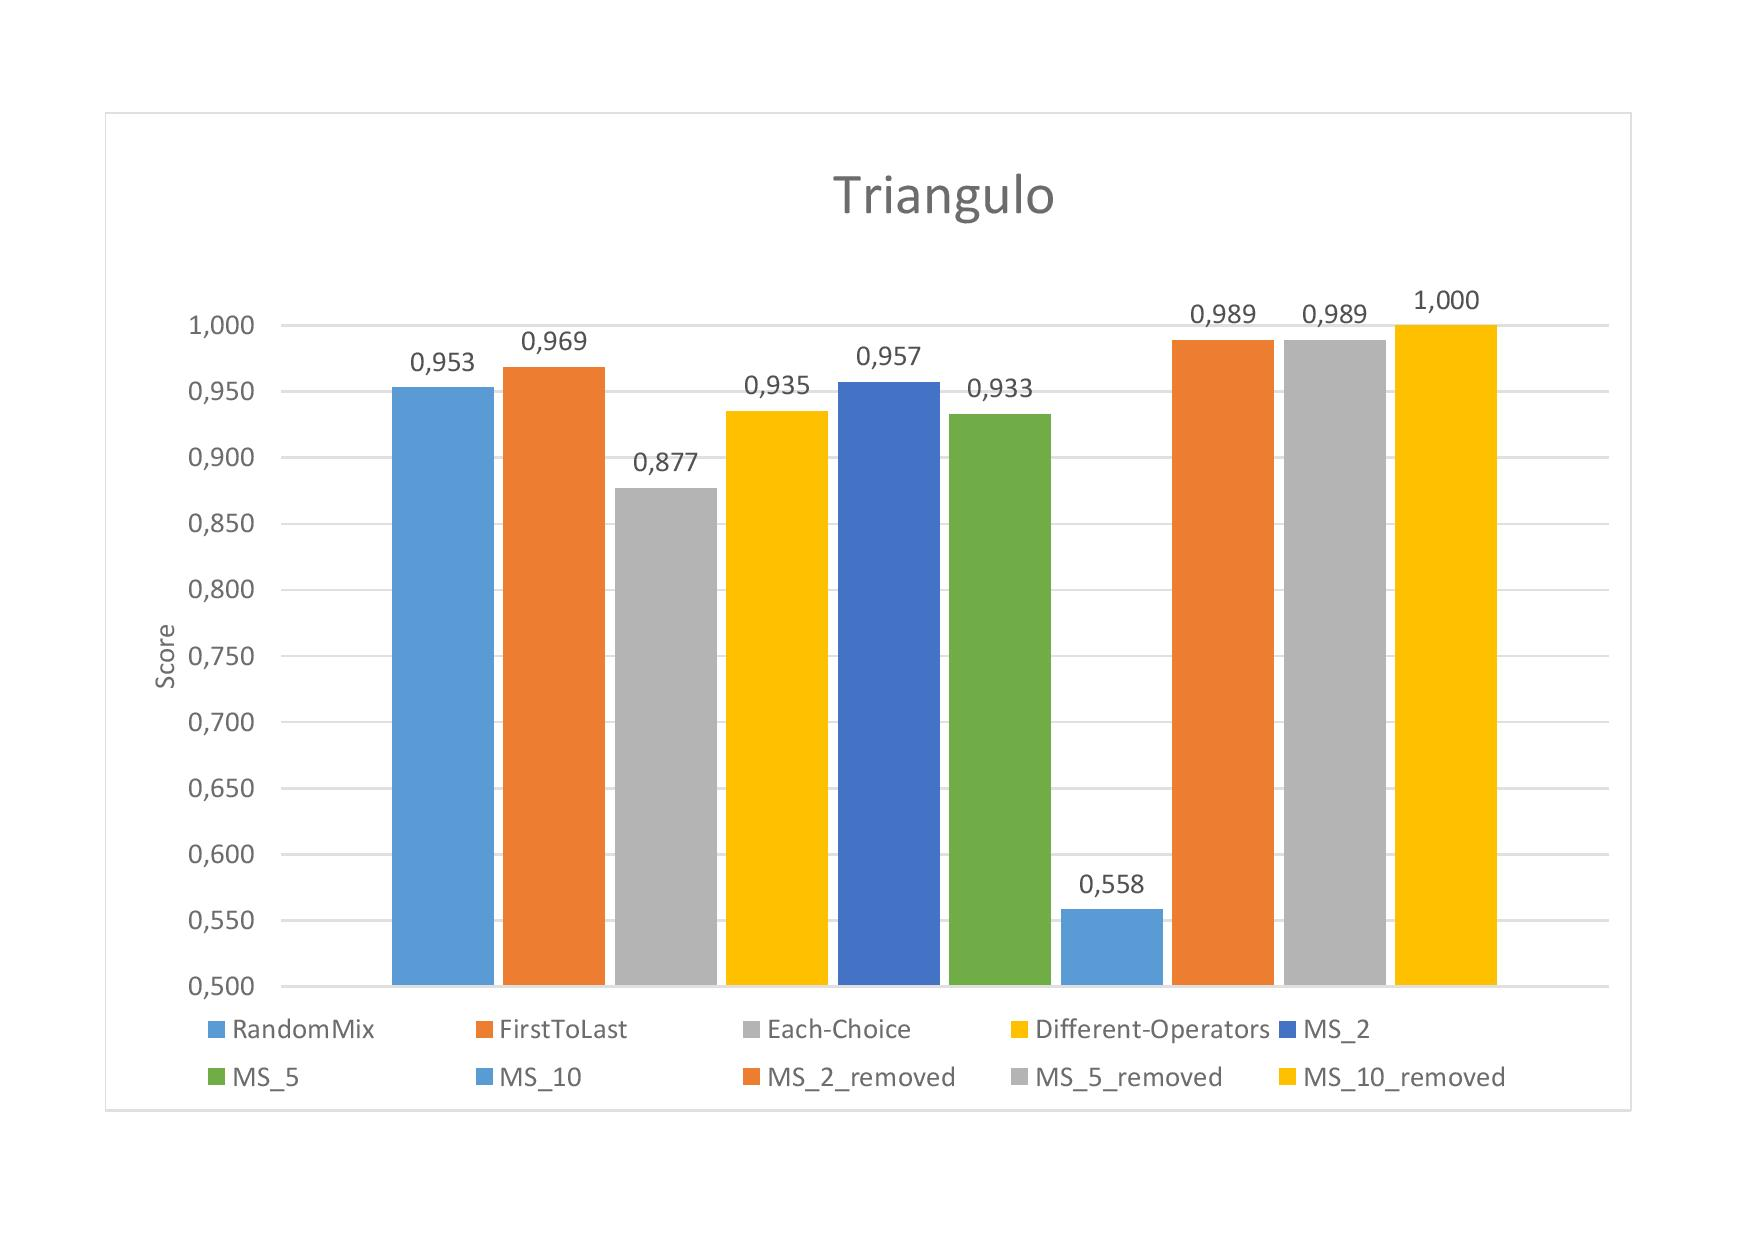
\includegraphics[width=1\textwidth]{graficos/problems/triangulo.jpg}
\caption{\textit{Scores} das estratégias no problema Triangulo}
\label{fig:triangulo}
\end{figure}
Assim como no problema anterior, neste a estratégia MS\_10 se mostra impraticável, enquanto as MS\_2 e MS\_5 mostram um desempenho muito próximo aos outros SOMs com melhores resultados. A MS\_2 teve desempenho inferior a somente a SOM First2Last. Algo interessante neste problema é o desempenho dos complementos de MS\_2 e MS\_5 com \textit{scores} próximos a 1.0.

\subsection{Análise por estratégia}
Nesta seção veremos o score em cada um dos problemas para cada estratégia escolhida assim como iremos fazer algumas comparações com base em alguns dados estatísticos disponíveis na tabela [\ref{tab:stats}] abaixo.
\begin{table}[ht]
\centering
\caption{Dados estatísticos sobre os \textit{scores} de cada estratégia em cada problema}
\label{tab:stats}
\begin{tabular}{|l|l|l|l|l|l|}
\hline
                             & \textbf{Mínimo} & \textbf{Máximo} & \textbf{Máximo-Mínimo} & \textbf{Média} & \textbf{Desvio padrão} \\ \hline
\textbf{RandomMix}           & 0.935           & 0.989           & 0.055                  & 0.961          & 0.016                  \\ \hline
\textbf{FirstToLast}         & 0.915           & 0.993           & 0.078                  & 0.959          & 0.024                  \\ \hline
\textbf{Each-Choice}         & 0.815           & 0.983           & 0.168                  & 0.926          & 0.061                  \\ \hline
\textbf{Different-Operators} & 0.935           & 0.995           & 0.061                  & 0.968          & 0.025                  \\ \hline
\textbf{MS\_2}               & 0.957           & 1.000           & 0.043                  & 0.981          & 0.017                  \\ \hline
\textbf{MS\_5}               & 0.933           & 1.000           & 0.067                  & 0.966          & 0.027                  \\ \hline
\textbf{MS\_10}              & 0.314           & 0.998           & 0.684                  & 0.664          & 0.255                  \\ \hline
\textbf{MS\_2\_removed}      & 0.904           & 0.998           & 0.095                  & 0.971          & 0.033                  \\ \hline
\textbf{MS\_5\_removed}      & 0.981           & 1.000           & 0.019                  & 0.992          & 0.007                  \\ \hline
\textbf{MS\_10\_removed}     & 1.000           & 1.000           & 0.000                  & 1.000          & 0.000                  \\ \hline
\end{tabular}
\end{table}

\subsubsection{Random}
\begin{figure}[H]
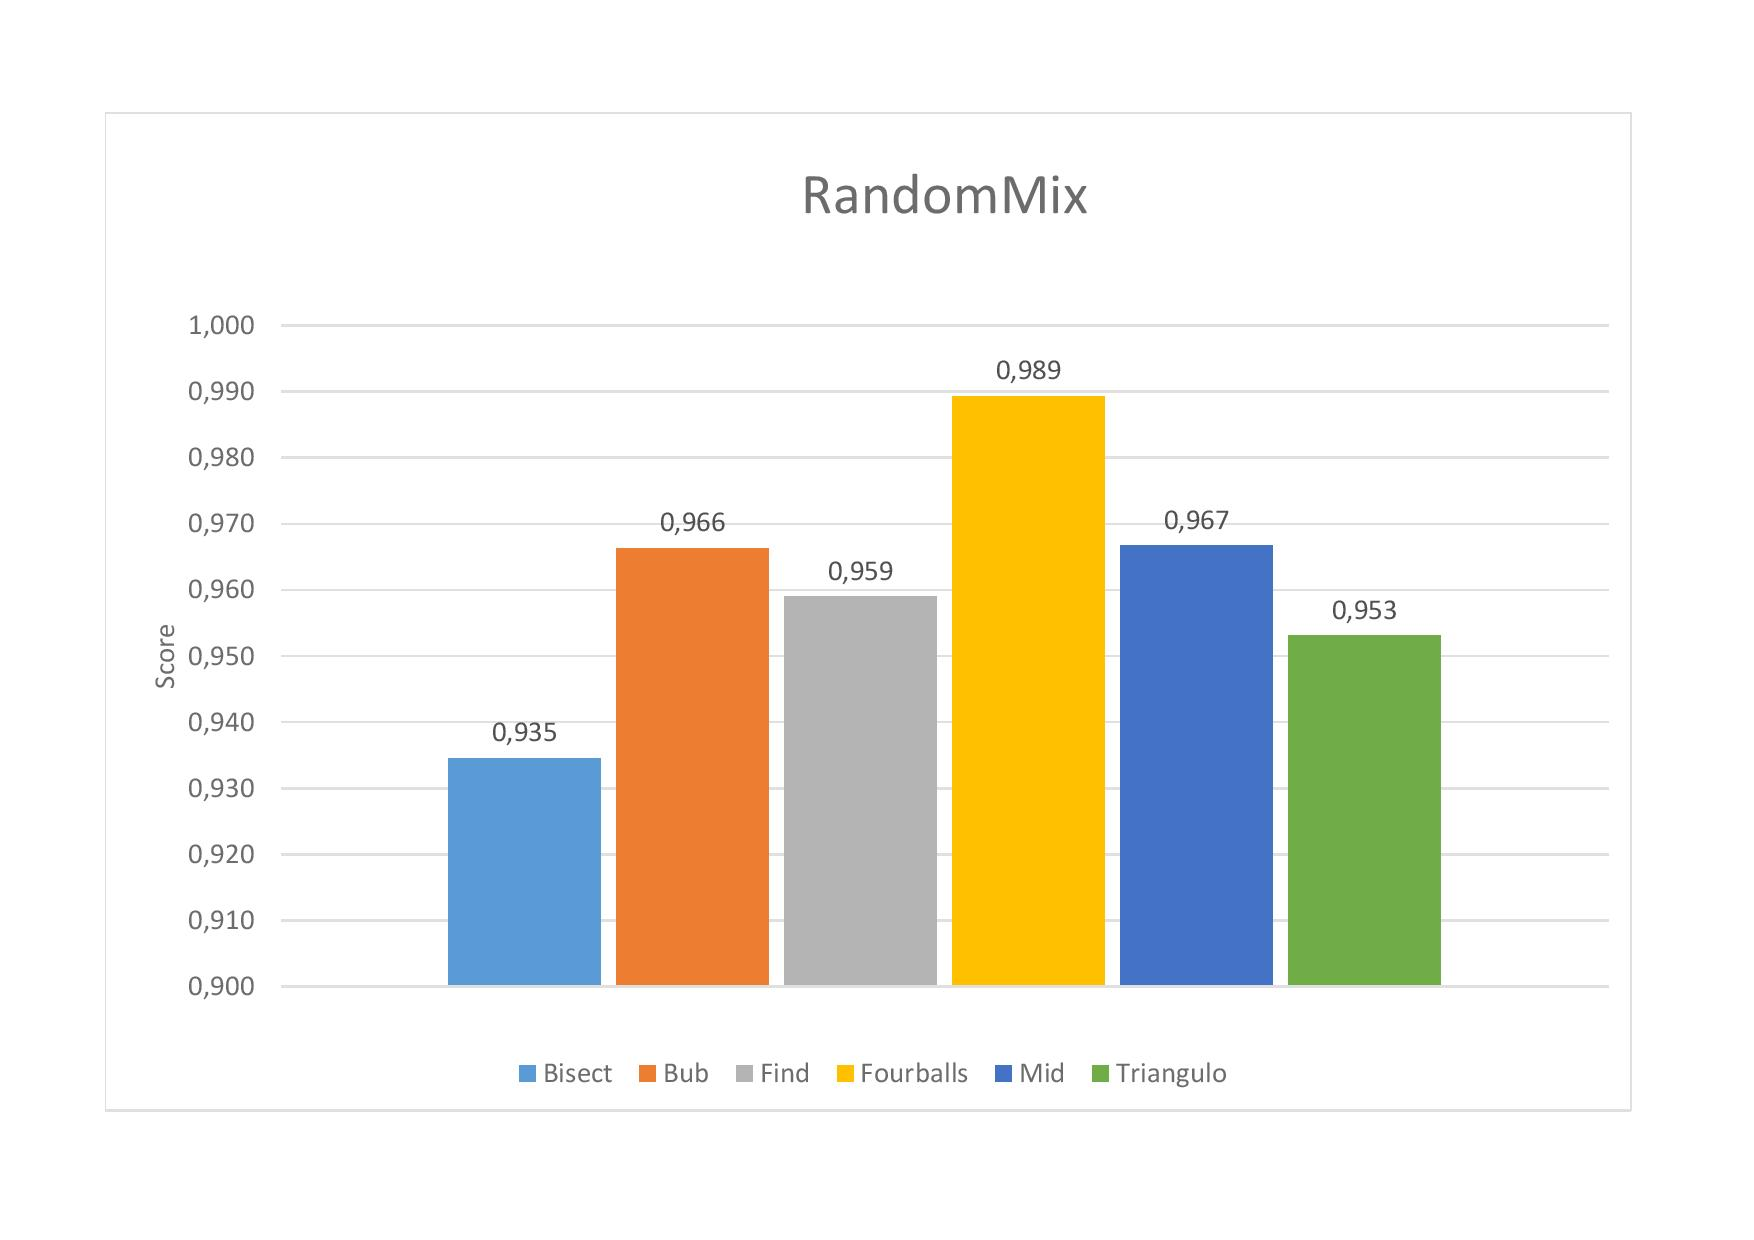
\includegraphics[width=1\textwidth]{graficos/strategies/randommix.jpg}
\caption{\textit{Scores} dos problemas usando a estratégia Random}
\label{fig:Random}
\end{figure}
Com o \textit{score} média média igual a 0.961 e desvio padrão a 0.016, podemos dizer que, no geral, esta estratégia parece ser uma solução razoável comparada às demais SOMs, porém ainda perdendo para as de Mutação seletiva.

\subsubsection{First2Last}
\begin{figure}[H]
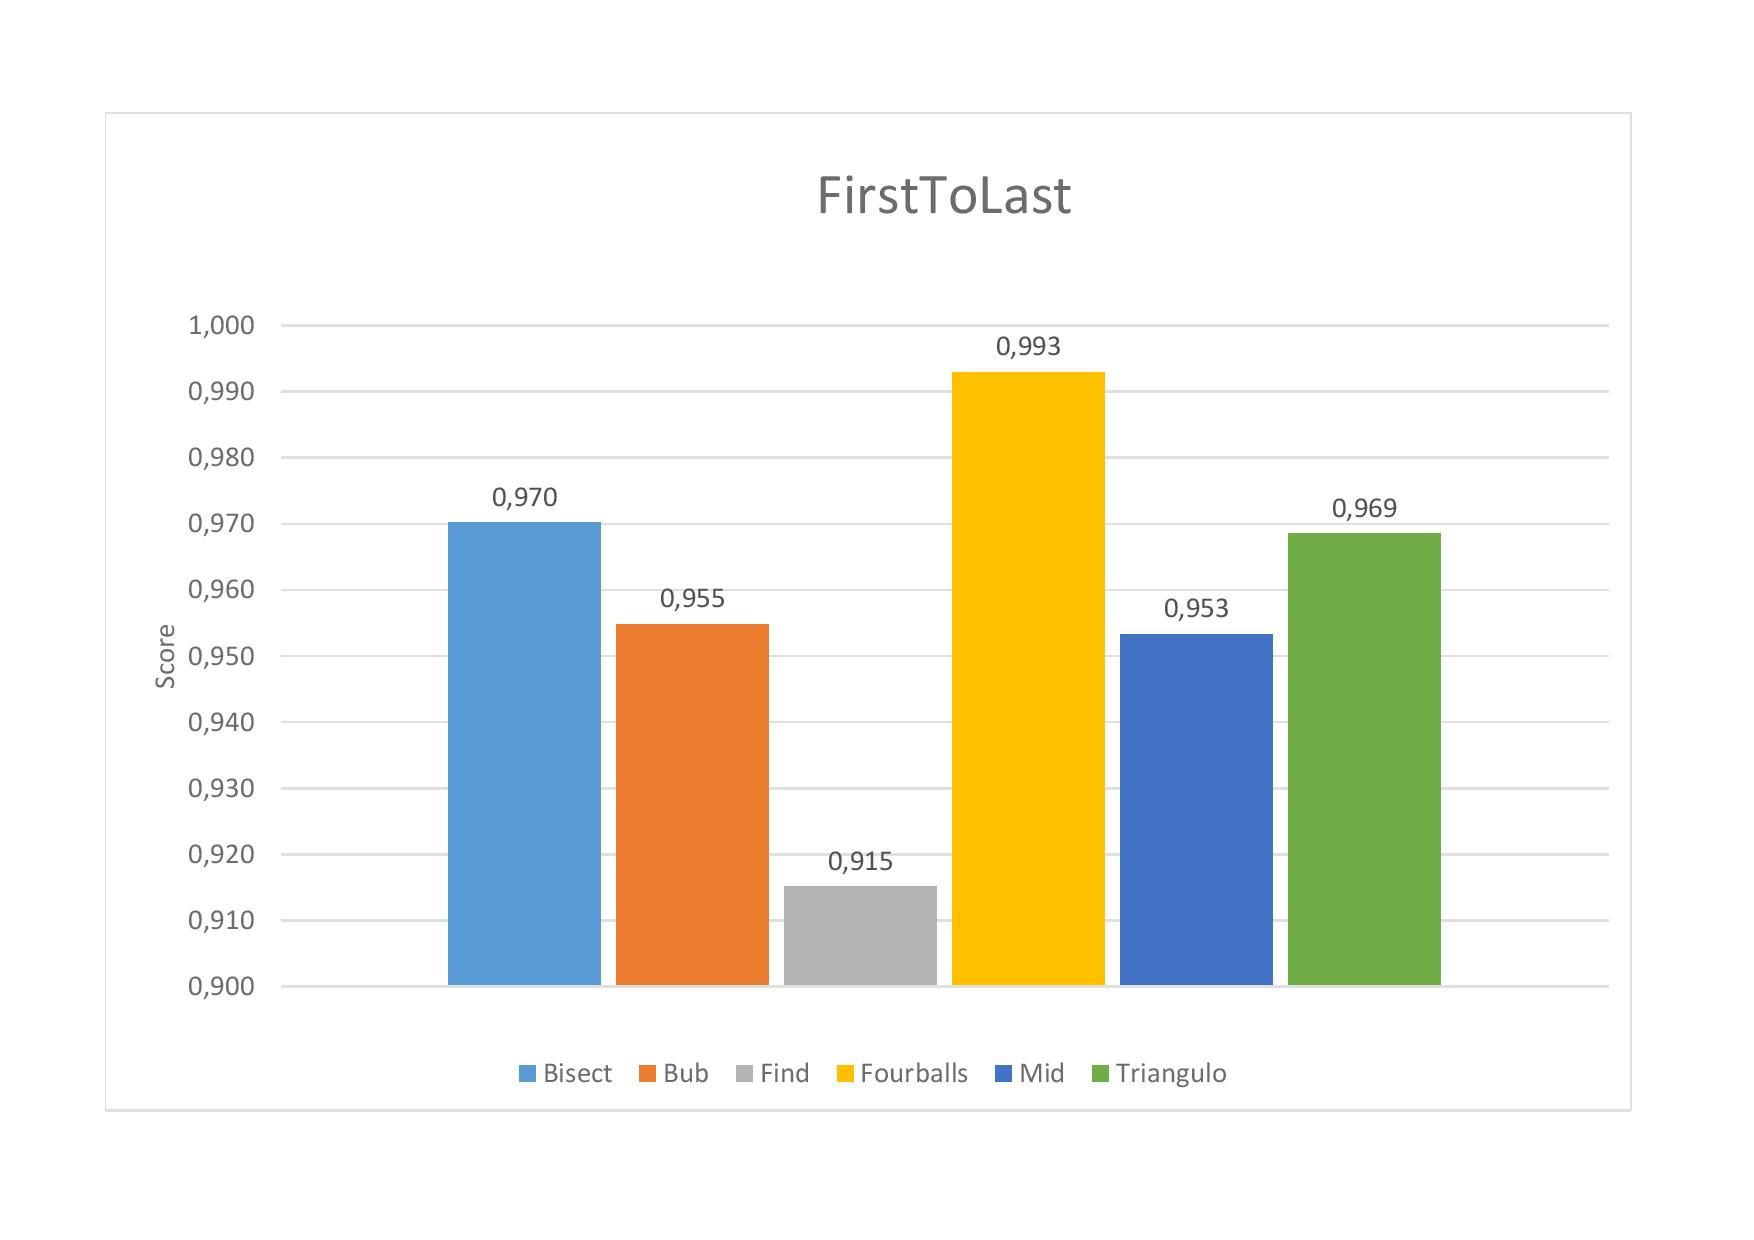
\includegraphics[width=1\textwidth]{graficos/strategies/firsttolast.jpg}
\caption{\textit{Scores} dos problemas usando a estratégia First2Last}
\label{fig:First2Last}
\end{figure}
Já a \textit{First2Last} mostra média menor (0.959) e desvio padrão maior (0.024) quando comparado à \textit{Random}, aparentando ser uma estratégia mais inconstante, no geral.

\subsubsection{Each-choice}
\begin{figure}[H]
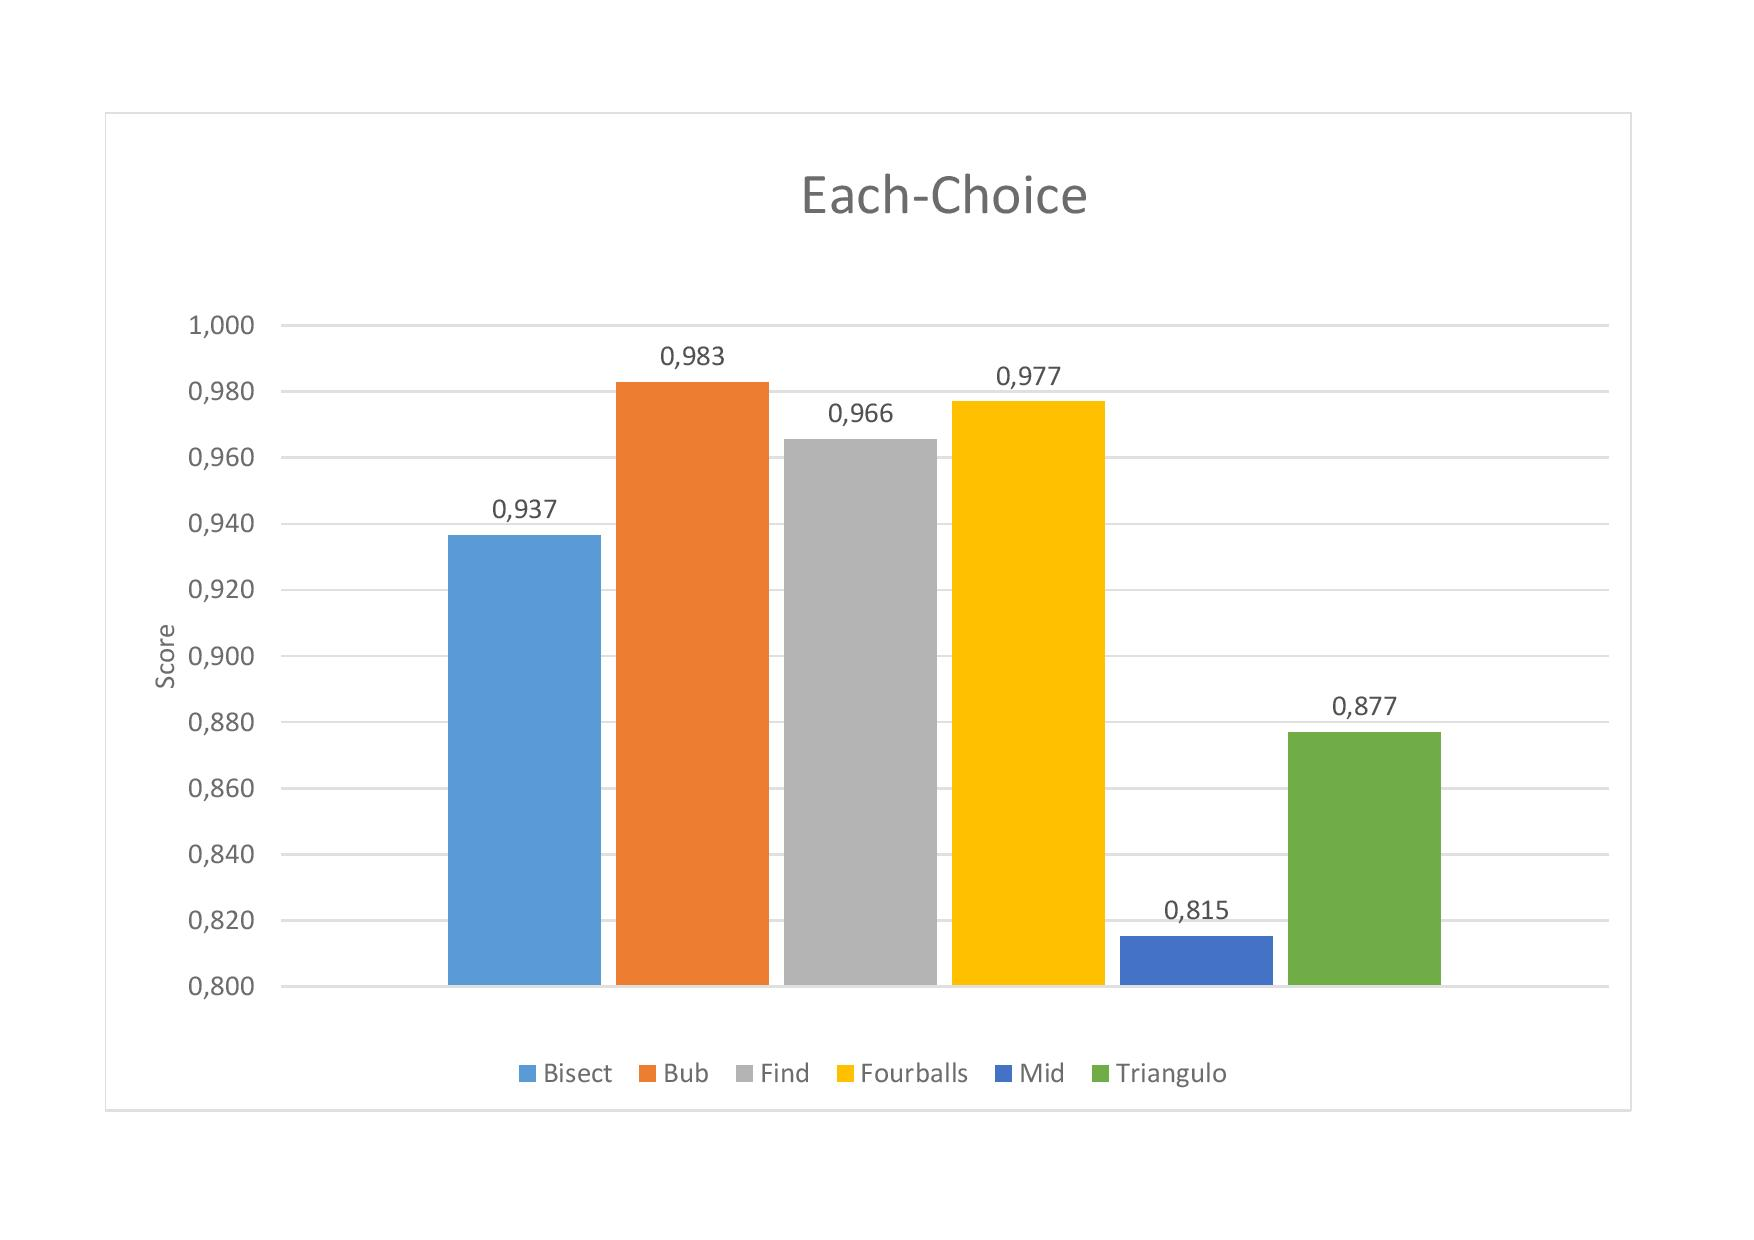
\includegraphics[width=1\textwidth]{graficos/strategies/each-choice.jpg}
\caption{\textit{Scores} dos problemas usando a estratégia Each-choice}
\label{fig:each-choice}
\end{figure}
A \textit{Each-choice} apresenta a maior diferença entre seu máximo e mínimo dentre os SOMs (0.168), a menor média (0.926) e maior desvio padrão, se mostrando ainda mais instável do que a \textit{First2Last}.

\subsubsection{Different-Operators}
\begin{figure}[H]
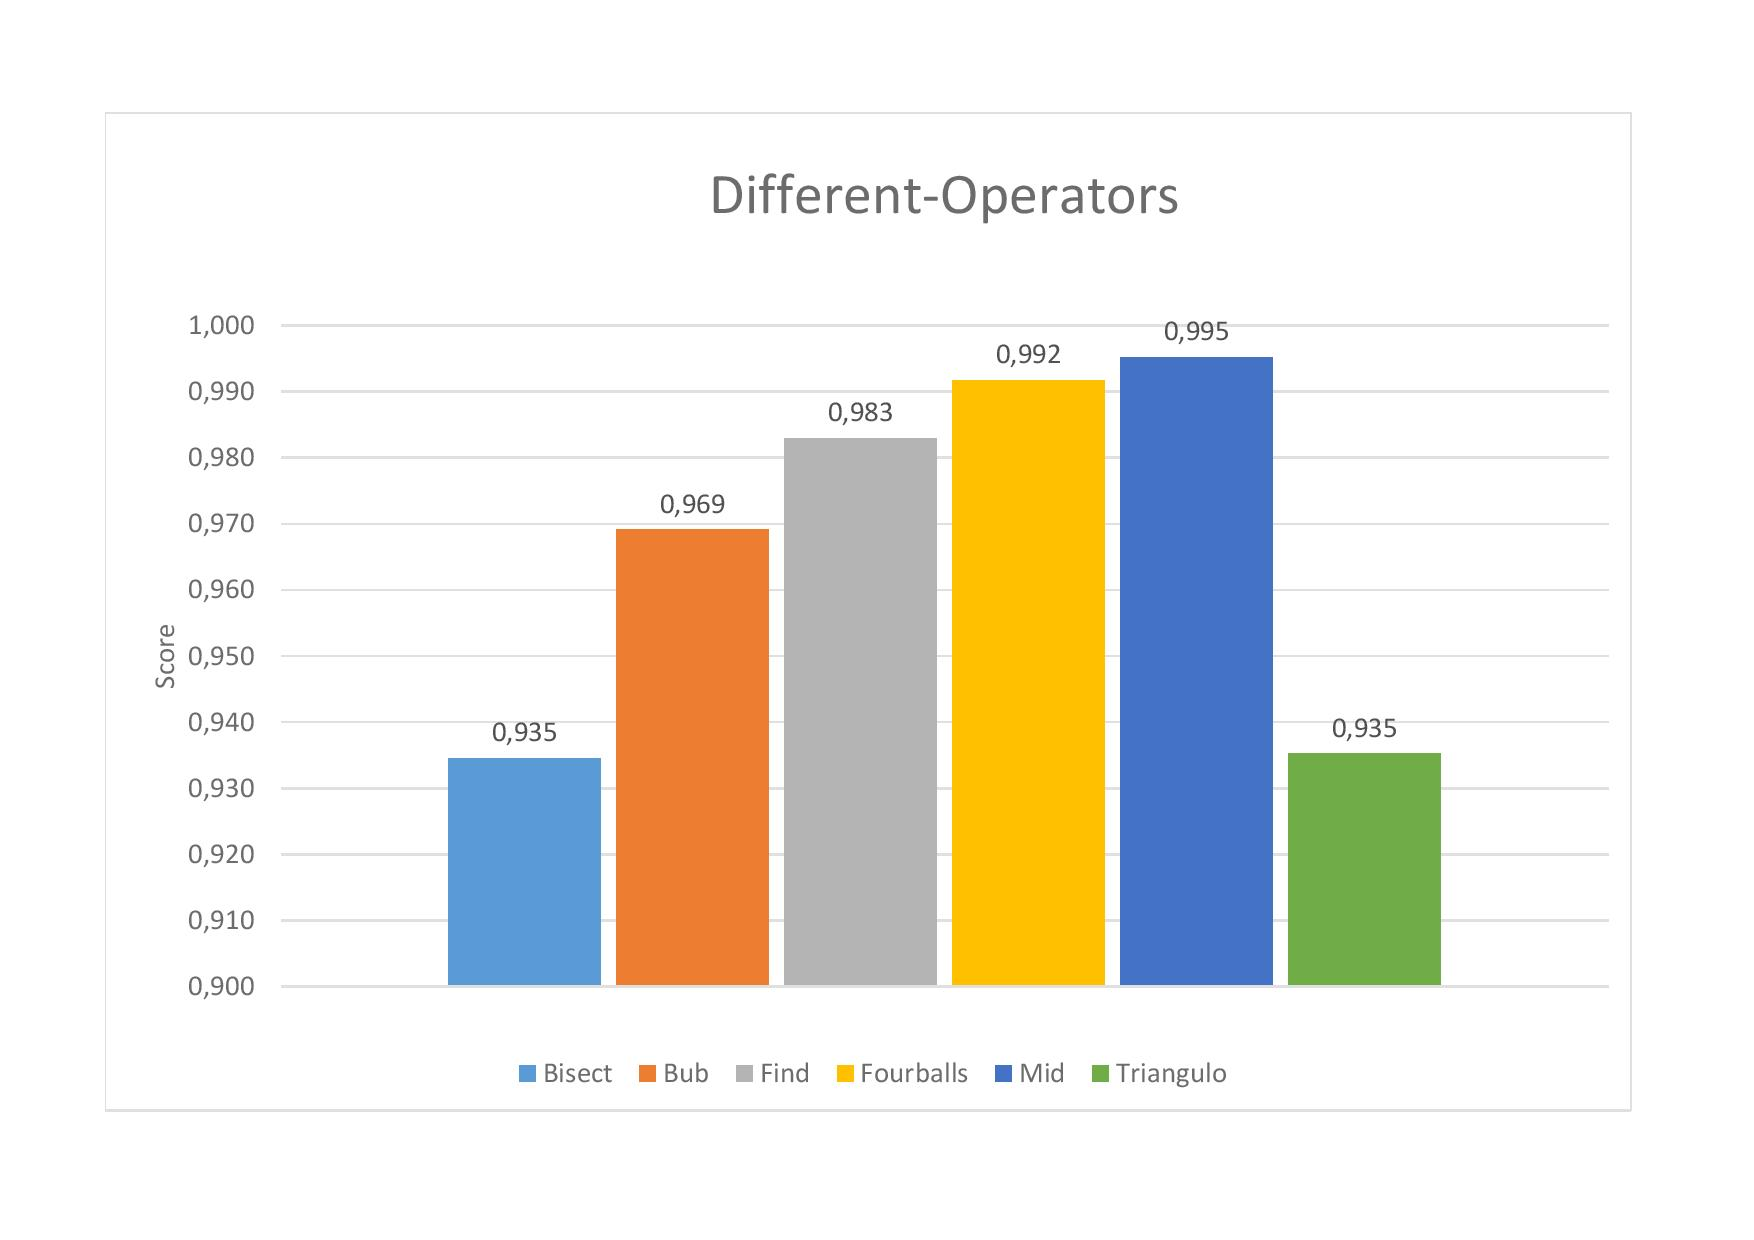
\includegraphics[width=1\textwidth]{graficos/strategies/different-operators.jpg}
\caption{\textit{Scores} dos problemas usando a estratégia Different-operators}
\label{fig:differente-operators}
\end{figure}
A \textit{Different-operators} apresentou a maior média (0.968) entre os SOMs, porém um desvio padrão elevado (0.025), no entando seus 2 maiores \textit{scores} ficaram príxmos de 1.0.

\subsubsection{Mutação seletiva}
\begin{figure}[H]
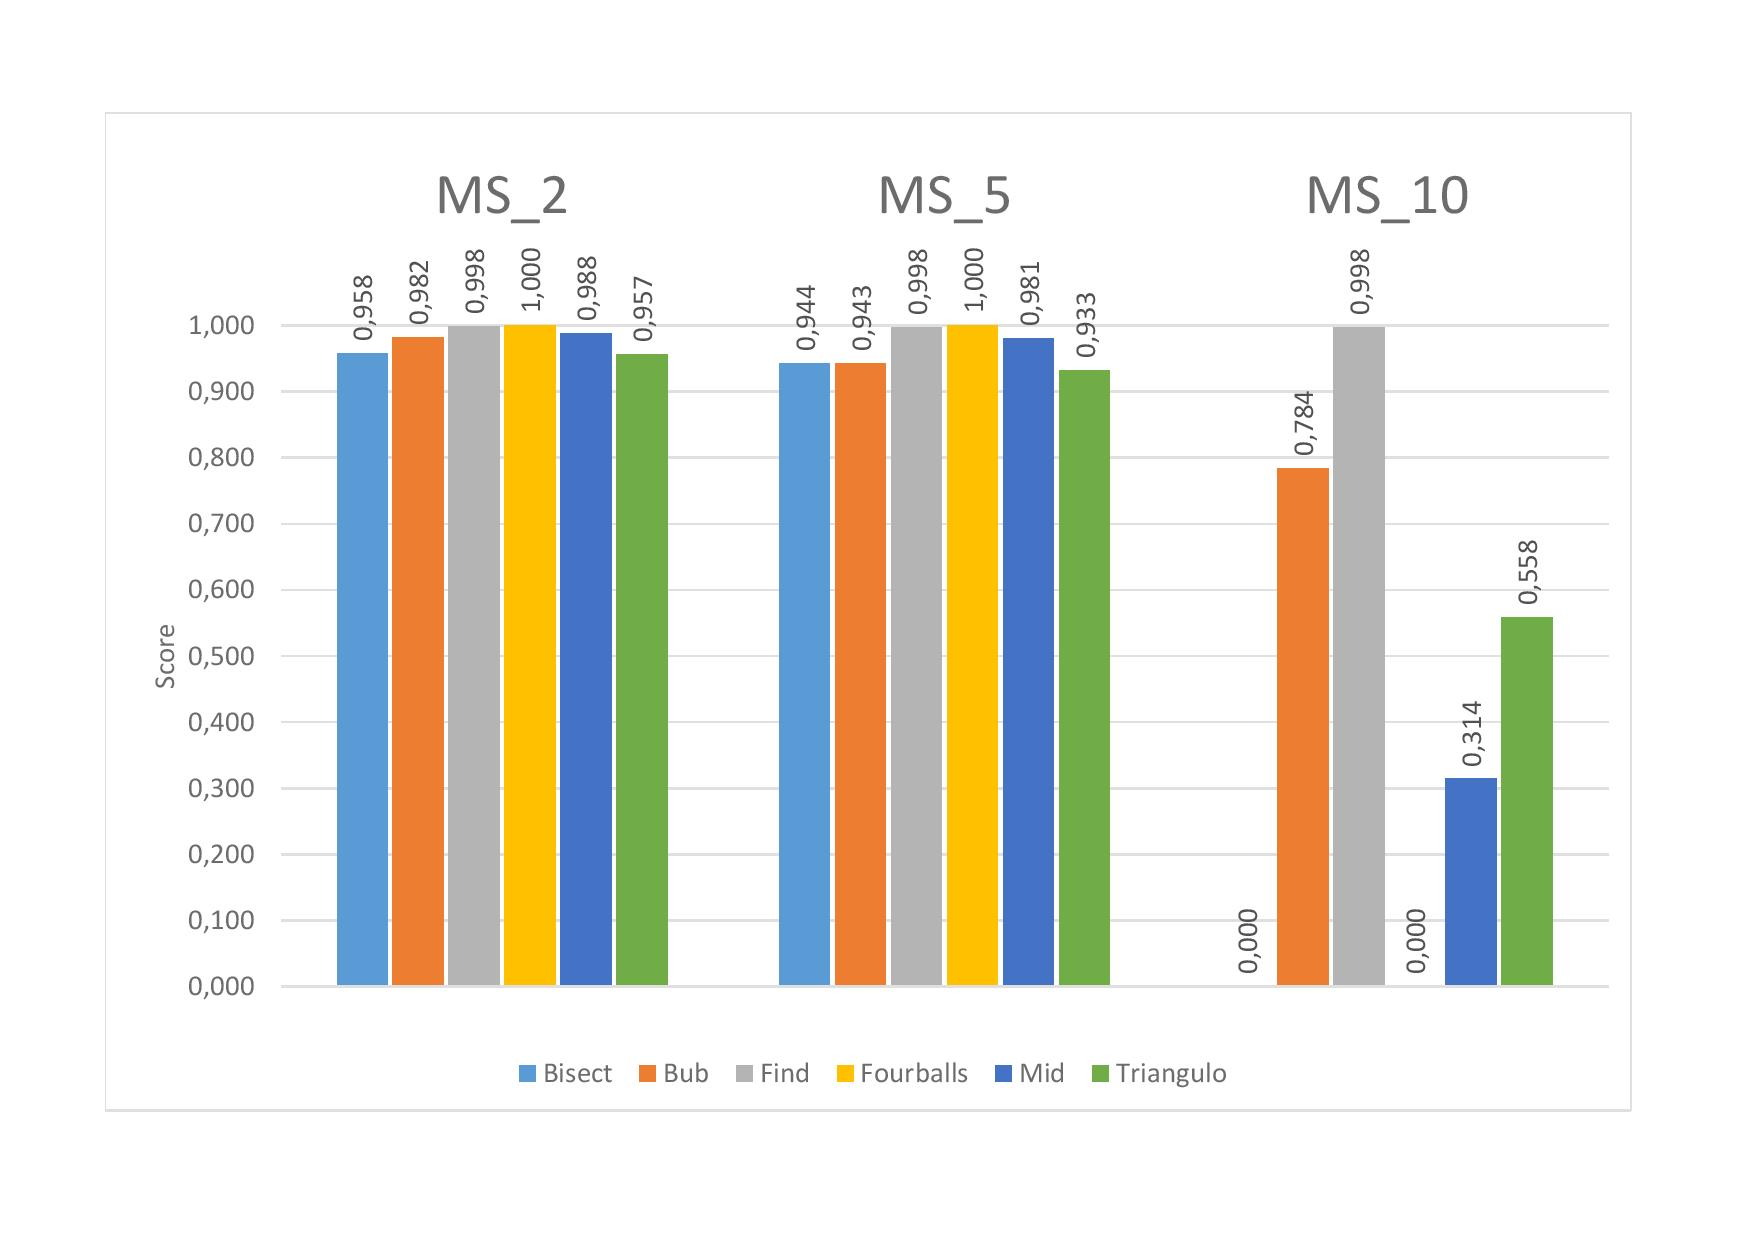
\includegraphics[width=1\textwidth]{graficos/strategies/mss.jpg}
\caption{\textit{Scores} dos problemas usando a estratégia Mutação seletiva}
\label{fig:selective}
\end{figure}
A estratégia MS\_2 apresentou resultados excelentes quando comparado aos SOMs, pois seu \textit{score} mínimo é maior que os dos SOMs e o máximo chegou a 1.0 no problema \textit{Fourballs}. Ainda sim podemos notar que dentre as estratégias de mutação seletiva, ele foi o que se mostrou mais estável com a maior média (0.981) e com desvio padrão igual a 0.017, perdendo por uma diferença menor que 0.001 para o melhor desvio padrão dos SOMs.

A estratégia MS\_5 também mostrou bons resultados, porém com maior variância entre os problemas. Assim como o MS\_2, obteve um \textit{score} máximo e outro muito próximo disso, nos mesmos problemas. Mesmo asism, sua média (0.966) ficou pior que apenas de uma estratégia SOM, a \textit{Different-operators} e com desvio padrão (0.027) maior do que 3 das estratégias SOM.

Já a estratégia MS\_10 se mostrou muito instável, pois em casos de ter poucos operadors na base inicial, restam poucos mutantes para os testes. Em dois dos problemas foram removidos todos os mutantes, porque a base inivial possuía menos de 10 operadores. Mesmo nos problemas onde sobraram mutantes para serem avaliados, seu desempenho ficou muito abaixo do esperado, com uma média de 0.664, a menor entre todas as estratégias avaliadas, e consequentemente o maior desvio padrão (0.255)

\subsubsection{Mutação seletiva - Complemento}
\begin{figure}[H]
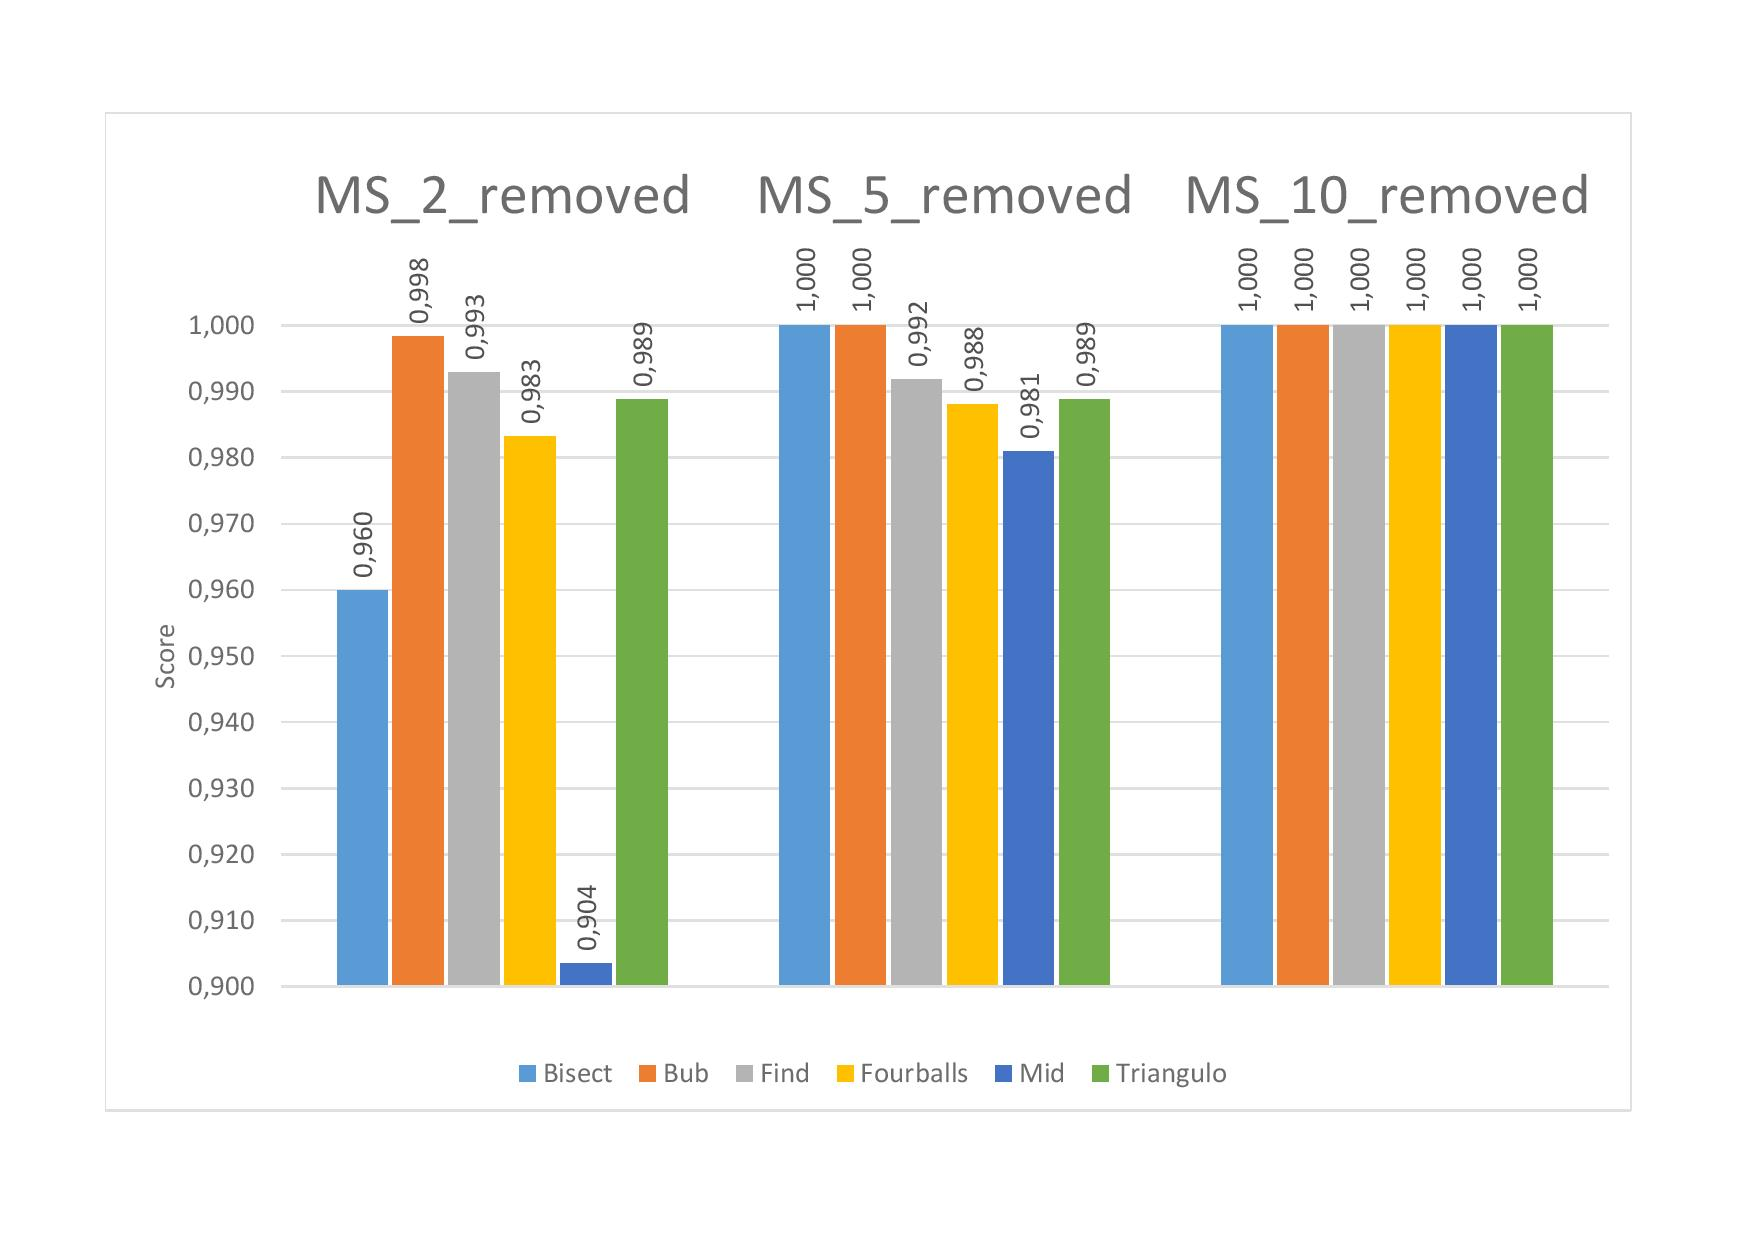
\includegraphics[width=1\textwidth]{graficos/strategies/mss_removed.jpg}
\caption{\textit{Scores} dos problemas usando a estratégia Mutação seletiva - Complemento}
\label{fig:selective-removed}
\end{figure}
As estratégias de mutantes removidos da mutação seletiva (complementares à ela) foram adicionados aos estudos por curiosidade e acabaram se mostrando bons resultados.

A estratégia MS\_2\_removed, mesmo com os mutantes de apenas 2 dos operadores das bases originais, mostrou resultados bons e próximos aos SOMs, com média de 0.971 mas com desvio padrão(0.033) elevado.

Algo surpreendente aconteceu ao ver os resultados da MS\_5\_removed, mesmo sendo apenas uma base complementar, ela se mostrou como a estratégia com \textit{scores} mais estáveis dentre todos os problemas, com média 0.992 e desvio padrão igual a 0.007. Seu \textit{score} mínimo foi de 0.981 (o maior dentre as estratégias apresentadas até agora) e o máximo 1.0. 

A estratégia MS\_10\_removed obteve \textit{scores} perfeitos em todos os problemas, porém em dois deles ele ficou com todos os FOMS e nos outros a maioria deles foi removida, o que acaba na verdade filtrando pouco a base inicial de FOMs, que era o proposto às estratégias.
\section{Conclusão}
\label{section:conclusao}
Este estudo apresentou a implementação da estratégia de Mutação Seletiva, 
assim como os resultados obtidos e uma análise breve sobre seus resultados
comparando-os aos mutantes de segunda ordem propostos.

Com os resultados apresentados, foi possível ver que algumas das 
estratégias de mutação seletiva apresentadas foram melhores ou no mínimo 
empataram ficaram equiparadas às estratégias de mutantes de segunda ordem.
Entretanto isso pode variar conforme o problema e quantidade de mutantes
gerados. No geral, vimos que a estratégia que obteve melhor desempenho
geral para os problemas propostos foi a MS\_5\_removed, que contém os 
mutantes retirados da mutação seletiva comum.

\section{Considerações Finais e Trabalhos futuros}
\label{section:future-work}
Algo que foi considerado ao fim desse estudo e análise, é que quando 
removemos uma quantidade muito grande de mutantes, o \textit{score}
final acaba sendo prejudicado, como ocorreu com a estratégia MS\_10. 

Algo que pode-se estudar para mitigar esse problema seria ao invés de
remover os mutantes gerados pelos \textit{X} operadores que geram mais
mutantes, calcular quantos operadores foram utilizados para gerar os 
mutantes de primeira ordem e retirar 10\%, 20\% ou 50\% desses operadores,
por exemplo, pois assim teremos a garantia que sempre restarão mutantes 
para serem avaliados.


\bibliographystyle{sbc}
\bibliography{sbc-template}

\end{document}